\documentclass[a4paper,11pt,oneside,onecolumn]{article}
\usepackage[utf8]{inputenc}
\usepackage{cmap}
\usepackage[T1]{fontenc}
\usepackage{beton}
\usepackage{eulervm}
\renewcommand{\sfdefault}{\rmdefault}
\usepackage[pdftex,colorlinks,citecolor=black,filecolor=black,linkcolor=black,urlcolor=black]{hyperref}
\usepackage{tikz}
\usetikzlibrary{positioning,arrows,automata,decorations.pathreplacing,decorations.text,decorations.markings,arrows,shapes,calc,fit}
\usepackage{caption}
\usepackage{subcaption}
\usepackage{multirow}
\usepackage{hhline}
\usepackage{graphicx}
\usepackage{amsmath}
\usepackage[noend]{algpseudocode}

\title{Homework 1}
\author{Mitar Milutinovic (24090156)}

\renewcommand\thesection{\arabic{section}.}
\renewcommand\thesubsection{\thesection (\alph{subsection})}

\begin{document}

\maketitle

\section{}

\subsection{}

$$ T_1(n) = O(n^2) $$

$$ T_2(n) = O(n^3) $$

\subsection{}

\begin{align*}
T(n) & = 32 T\left(\frac{n}{4}\right) + 67 O\left( \left(\frac{n}{4}\right)^2 \right) = \\
     & = 32 T\left( \frac{n}{4} \right) + O\left( n^2 \right) = \\
     & = O\left( n^{\log_4 32} \right) = O\left(n^{2.5}\right) \\
\end{align*}

\subsection{}

\begin{center}
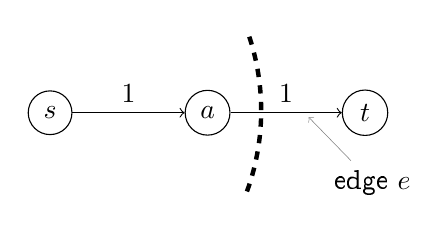
\begin{tikzpicture}

\node[draw, circle] (s) at (0,0) {$s$};
\node[draw, circle] (a) at (2,0) {$a$};
\node[draw, circle] (t) at (4,0) {$t$};
\draw[->] (s) -- node[above] {$1$} (a);
\draw[->] (a) -- node[above,pin={[pin distance=20pt,pin edge={<-,shorten <=3pt}]-60:edge $e$}] {$1$} (t);

\draw[ultra thick,dashed] (2.5,-1) arc (-20:20:3);

\end{tikzpicture}
\end{center}

Max-flow solution for the graph above has a minimum cut which contains an edge $e$ with capacity $1$.
But even if we increase capacity of the edge $e$, max flow does not increase. Thus, the problem statement
does not hold by counterexample.

\subsection{}

\begin{alignat*}{6}
 & & &        & &        & \llap{$\max z$} & & \\
-x  & {}-{} & y & & & {}+{} & z & {}\le{} & 0 \\
& {}-{} & y  & {}-{} & w & {}+{} & z & {}\le{} & 0 \\
-3x & & & {}-{} & w & {}+{} & z & {}\le{} & 0 \\
x & {}+{} & y & {}+{} & w & & & {}={} & 1 \\
 & & &        & &        & \llap{$x,y,w$} & {}\ge{} & 0 \\
\end{alignat*}

\subsection{}

We relax $\forall v \in V, x_v \in \{0,1\}$ into $\forall v \in V, x_v \ge 0$. Solving the linear program gives us $\tilde{x}_v$.
Vertex cover of $G$ is $S = \left\{ v | \tilde{x}_v \ge \frac{1}{2} \right\} $. $S$ is a 2-approximation for the optimal vertex cover of $G$.

\subsection{}

$$ A = C\left( f(s_I), t \right) + v_I $$
$$ B = C\left( t, f(s_I) \right) + v_I $$

\subsection{}

$ O(nE) $, where $ E = \max_i e_i $, the finishing time of the last job.

\section{}

\subsection{}

\begin{algorithmic}
\Function{NotDominate}{$A$}
    \If{$|A| = 1$}
        \State \Return $A$
    \Else
        \State $B \gets $ \Call{NotDominate}{$A[0..(\frac{|A|}{2}-1)]$}
        \State $C \gets $ \Call{NotDominate}{$A[\frac{|A|}{2}..(|A|-1)]$}
        \State $R \gets []$
        \For{$b$ in $B$}
            \If{$b$ is not dominated by any $p$ in $C$}
                \State $R \gets R + [b]$
            \EndIf
        \EndFor
        \State $R \gets R + C$

        \State \Return $R$
    \EndIf
\EndFunction

\vspace{2em}

\end{algorithmic}

\begin{algorithmic}
\State $A \gets $ sort $S$ by $x$ coordinate in the ascending order
\State \Return \Call{NotDominate}{$A$}
\end{algorithmic}

\subsection{}

\begin{algorithmic}
\State $A \gets $ sort $S$ by $x$ coordinate in the decreasing order
\State find the longest increasing subsequence of $y$ coordinates of points in $A$
\State \Return{points of the longest increasing subsequence}
\end{algorithmic}

\section{}

Each clause $C_j$ contains three variables, $x_i$ or $\bar{x}_i$. Each clause vertex $c_j$ corresponds to clause $C_j$.
Each variable vertex $v_i$ corresponds to variable $x_i$, $v'_i$ to variable $\bar{x}_i$. We connect every $c_j$ to all $v_i$ and $v'_i$
except $v_i$ if $x_i \in C_j$ and $v'_i$  if $\bar{x}_i \in C_j$. We color the graph with $k = n+1$ colors.

\section{}

\subsection{}

\begin{algorithmic}
\State $r \gets \{\}$
\For{$ i = 0 \to (n-(m-1)-1) $}
    \State $z \gets 0$
    \For{$j = 0 \to m-1$}
        \If{$s_2[i + j] \ne s_1[j]$}
            \State $z \gets z + 1$
        \EndIf
    \EndFor
    \If{$z \le k$}
        \State $r \gets r \cup \{i\}$
    \EndIf
\EndFor
\State \Return $r$
\end{algorithmic}

\subsection{}

\begin{algorithmic}
\State $r \gets \{\}$
\State $s_1 \gets (s_1 - 0.5) \cdot 2$  
\State $s_2 \gets (s_2 - 0.5) \cdot 2$  
\State $S_1 \gets $ \Call{FFT}{$s_1$}
\State $S_2 \gets $ \Call{FFT}{$s_2$}
\State $C \gets S_1 \cdot $ \Call{Reverse}{$S_2$} \Comment{correlation}
\State $c \gets $ \Call{FFT}{$C$} \Comment{$c$ is of length $n + m - 1$}
\For{$ i = m -1 \to n - 1 $}
    \If{$c[i] \ge m - 2 \cdot k$}
        \State $r \gets r \cup \{i - (m - 1)\}$
    \EndIf
\EndFor
\State \Return $r$
\end{algorithmic}

\section{}

\subsection{}

$$ b(\pi) / 2 $$

\subsection{}

\begin{algorithmic}
\While{$b(\pi) > 0$}
    \ForAll{$\pi_i\dots\pi_j$ between two breakpoints}
        \If{$\rho(i, j)$ removes more breakpoints of $\pi$ than $\rho$}
            \State $\rho \gets \rho(i, j)$
        \ElsIf{$\rho(i, j)$ removes equal number breakpoints of $\pi$ as $\rho$}
            \If{$\pi_i\dots\pi_j$ is increasing}
                \State $\rho \gets \rho(i, j)$            
            \EndIf
        \EndIf
    \EndFor
    \State $\pi \gets \pi \circ \rho$
\EndWhile
\State \Return $\pi$
\end{algorithmic}

\end{document}
